%%%%%%%%%%%%%%%%%%%%%%%%%%%%%%%%%%%%%%%%%%%%%%%%%%%%%%%%%%%%%%%%%%%%%%%
%%%%%%%%%%%%%%%%%%%%%%%%%%%%%%%%%%%%%%%%%%%%%%%%%%%%%%%%%%%%%%%%%%%%%%%
%%%%%                                                                 %
%%%%%     <file_name>.tex                                             %
%%%%%                                                                 %
%%%%% Author:      <author>                                           %
%%%%% Created:     <date>                                             %
%%%%% Description: <description>                                      %
%%%%%                                                                 %
%%%%%%%%%%%%%%%%%%%%%%%%%%%%%%%%%%%%%%%%%%%%%%%%%%%%%%%%%%%%%%%%%%%%%%%
%%%%%%%%%%%%%%%%%%%%%%%%%%%%%%%%%%%%%%%%%%%%%%%%%%%%%%%%%%%%%%%%%%%%%%%

%%%%%%%%%%%%%%%%%%%%%%%%%%%%%%%%%%%%%%%%%%%%%%%%%%%%%%%%%%%%%%%%%%%%%%%
%%%%%                                                                 %
%%%%%     Document Class                                              %
%%%%%                                                                 %
%%%%%%%%%%%%%%%%%%%%%%%%%%%%%%%%%%%%%%%%%%%%%%%%%%%%%%%%%%%%%%%%%%%%%%%
\documentclass[%
 oneside,      % Use the same margins for odd and even pages (cannot
               % be used with the 'twoside' option). 
% twoside,      % Use different margins for odd and even pages (cannot
               % be used with the 'oneside' option).
 openany,      % Open chapters on odd and even pages.
 halfparskip,  % Create small spaces for new paragraphs but no indents.
]{scrbook}

%%%%%%%%%%%%%%%%%%%%%%%%%%%%%%%%%%%%%%%%%%%%%%%%%%%%%%%%%%%%%%%%%%%%%%%
%%%%%                                                                 %
%%%%%     Preamble                                                    %
%%%%%                                                                 %
%%%%%%%%%%%%%%%%%%%%%%%%%%%%%%%%%%%%%%%%%%%%%%%%%%%%%%%%%%%%%%%%%%%%%%%
% Load the preamble from another file.
%%%%%%%%%%%%%%%%%%%%%%%%%%%%%%%%%%%%%%%%%%%%%%%%%%%%%%%%%%%%%%%%%%%%%%%
%%%%%%%%%%%%%%%%%%%%%%%%%%%%%%%%%%%%%%%%%%%%%%%%%%%%%%%%%%%%%%%%%%%%%%%
%%%%%                                                                 %
%%%%%     preamble.tex                                                %
%%%%%                                                                 %
%%%%% Author:      Michael Muehlberghuber                             %
%%%%% Created:     01.07.2012                                         %
%%%%% Description: This file contains the preamble of the             %
%%%%%              Semester-/Master-Project LaTeX report example.     %
%%%%%                                                                 %
%%%%% History:                                                        %
%%%%%%%%%%%%%%                                                        %
%%%%% 2012/07/01:  *) Created initial version.                        %
%%%%%                                                                 %
%%%%%%%%%%%%%%%%%%%%%%%%%%%%%%%%%%%%%%%%%%%%%%%%%%%%%%%%%%%%%%%%%%%%%%%
%%%%%%%%%%%%%%%%%%%%%%%%%%%%%%%%%%%%%%%%%%%%%%%%%%%%%%%%%%%%%%%%%%%%%%%

%%%%%%%%%%%%%%%%%%%%%%%%%%%%%%%%%%%%%%%%%%%%%%%%%%%%%%%%%%%%%%%%%%%%%%%
%%%%%                                                                 %
%%%%%     Package Loading                                             %
%%%%%                                                                 %
%%%%%%%%%%%%%%%%%%%%%%%%%%%%%%%%%%%%%%%%%%%%%%%%%%%%%%%%%%%%%%%%%%%%%%%

% Determines the input encoding.
\usepackage[%
 utf8,
% latin1
]{inputenc}

% ---------------------------------------------------------------------

% Determines the output encoding.
\usepackage[T1]{fontenc}

% ---------------------------------------------------------------------

% Determines language settings.
\usepackage[%
 english    % You may change this to 'ngerman' in order to write a
            % german report.
]{babel}

% ---------------------------------------------------------------------

% Provides image loading.
\usepackage{graphicx}

% ---------------------------------------------------------------------

% Provides customization of chapter headings.
\usepackage[%
	Lenny     % Choose a nice layout for chapter headings.
]{fncychap}

% ---------------------------------------------------------------------

% Provides some blindtext.
\usepackage{lipsum}

% ---------------------------------------------------------------------

% Provides stretchable tables.
\usepackage{tabularx}

% ---------------------------------------------------------------------

% Provides some fancy boxes.
\usepackage{fancybox}

% ---------------------------------------------------------------------

% Provides subfigures.
\usepackage{subfig}

% ---------------------------------------------------------------------

% Provides colors in LaTeX.
\usepackage{xcolor}

% ---------------------------------------------------------------------

% Provides conditionals (for titlepage).
\usepackage{xifthen}

% ---------------------------------------------------------------------

% Provides the algorithm environment
\usepackage[ruled,%
            linesnumbered]{algorithm2e}

% ---------------------------------------------------------------------

% Provides bold greek math symbols.
\usepackage{bm}

% ---------------------------------------------------------------------

% Allows to include pdf documents.
\usepackage{pdfpages}

% ---------------------------------------------------------------------

% Provides nicer tables than the standard tables.
\usepackage{booktabs}

% ---------------------------------------------------------------------

% Provides simple line spacings.
\usepackage{setspace}

% ---------------------------------------------------------------------

% Provides simple line spacings.
\usepackage{geometry}

% ---------------------------------------------------------------------

% Provides more customizeable captions.
\usepackage{capt-of}

% ---------------------------------------------------------------------

% Provides small table of contents (e.g., for single chapters or the
% appendix).
\usepackage{minitoc}

% ---------------------------------------------------------------------

% Provides a simple command to describe a directory tree.
\usepackage{dirtree}

% ---------------------------------------------------------------------

%%%%%                                                             %%%%%
%%%%% ATTENTION: Loading further packagaes should go in here.     %%%%%
%%%%%                                                             %%%%%

% ---------------------------------------------------------------------

% Provides hyperlinks within your document. Should always be loaded at
% the end.
\usepackage{hyperref}

% ---------------------------------------------------------------------

% Provides multiple glossaries (incl. list acronyms, list of symbols,
% etc.).
\usepackage[%
 toc,              % Add the glossaries to the table of contents.
 acronym,          % Add a list of acronyms.
 section=chapter,  % Show glossary headers as chapters.
 nonumberlist,     % Do not print the page numbers next to glossary
                   % entries.
]{glossaries}



%%%%%%%%%%%%%%%%%%%%%%%%%%%%%%%%%%%%%%%%%%%%%%%%%%%%%%%%%%%%%%%%%%%%%%%
%%%%%                                                                 %
%%%%%     Custom Settings                                             %
%%%%%                                                                 %
%%%%%%%%%%%%%%%%%%%%%%%%%%%%%%%%%%%%%%%%%%%%%%%%%%%%%%%%%%%%%%%%%%%%%%%
% Do not use sans-serif fonts for all dispositions (chapters,
% sections, etc.)
\setkomafont{disposition}{\normalfont\bfseries}


%%%%%%%%%%%%%%%%%%%%%%%%%%%%%%%%%%%%%%%%%%%%%%%%%%%%%%%%%%%%%%%%%%%%%%%
%%%%%                                                                 %
%%%%%     Custom Macros                                               %
%%%%%                                                                 %
%%%%%%%%%%%%%%%%%%%%%%%%%%%%%%%%%%%%%%%%%%%%%%%%%%%%%%%%%%%%%%%%%%%%%%%
% Create an inline command for shell commands.
\newcommand{\shell}[1]{\texttt{#1}}

% Create an enviroment for a shell commands.
\newenvironment{shellenv}%
{\VerbatimEnvironment%
 \begin{Sbox}\begin{minipage}{0.97\textwidth}\begin{Verbatim}%
}%
{\end{Verbatim}\end{minipage}\end{Sbox}%
\setlength{\fboxsep}{6pt}\shadowbox{\TheSbox}}%

% Create an inline command for files.
\newcommand{\file}[1]{\texttt{#1}}

% Create a command for command parameters.
\newcommand{\parameter}[1]{$<$#1$>$}


%%%%%%%%%%%%%%%%%%%%%%%%%%%%%%%%%%%%%%%%%%%%%%%%%%%%%%%%%%%%%%%%%%%%%%%
%%%%%                                                                 %
%%%%%     Titlepage Macros - !!! DO NOT CHANGE !!!                    %
%%%%%                                                                 %
%%%%%%%%%%%%%%%%%%%%%%%%%%%%%%%%%%%%%%%%%%%%%%%%%%%%%%%%%%%%%%%%%%%%%%%
% Create a command for missing title page parameters.
\newcommand{\misspar}[1]{\textcolor{red}{\textbf{$<$#1$>$}}}

\makeatletter

% Redefine existing class macros as missing.
\title{\misspar{Specify Title}}%
\author{\misspar{Specify Author}}%
\date{\misspar{Specify Date}}%

% Define a command for setting the semester on the titlepage.
\def\@semester{\misspar{Specify Semester}}%
\newcommand{\setsemester}[1]{\def\@semester{#1}}%
\let\semester\setsemester%
\newcommand{\show@semester}{\@semester}%

% Define a command for setting the type of the report (Master Thesis,
% Semester Project, etc.) on the titlepage.
\def\@reporttype{\misspar{Specify Report Type}}%
\newcommand{\setreporttype}[1]{\def\@reporttype{#1}}%
\let\reporttype\setreporttype%
\newcommand{\show@reporttype}{\@reporttype}%

% Define a command for setting the image path for the image on the
% titlepage.
\def\@titlelogo{}%
\newcommand{\settitlelogo}[1]{\def\@titlelogo{#1}}%
\let\titlelogo\settitlelogo%

% Define a command for setting the image height on the titlepage.
\def\@logoheight{7cm}%
\newcommand{\setlogoheight}[1]{\def\@logoheight{#1}}%
\let\logoheight\setlogoheight%
\newcommand{\show@logoheight}{\@logoheight}%

% Define a command for setting the email on the titlepage.
\def\@email{\misspar{Specify E-Mail}}%
\newcommand{\setemail}[1]{\def\@email{#1}}%
\let\email\setemail%
\newcommand{\show@email}{\@email}%

% Define a command for setting the first supervisor on the titlepage.
\def\@firstsup{\misspar{Specify First Supervisor}}%
\newcommand{\setfirstsup}[1]{\def\@firstsup{#1}}%
\let\firstsup\setfirstsup%
\newcommand{\show@firstsup}{\@firstsup}%

% Define a command for setting the second supervisor on the titlepage.
\def\@secondsup{\misspar{Specify Second Supervisor}}%
\newcommand{\setsecondsup}[1]{\def\@secondsup{#1}}%
\let\secondsup\setsecondsup%
\newcommand{\show@secondsup}{\@secondsup}%

% Define a command for setting the professor on the titlepage.
\def\@professor{\misspar{Specify Professor}}%
\newcommand{\setprofessor}[1]{\def\@professor{#1}}%
\let\professor\setprofessor%
\newcommand{\show@professor}{\@professor}%

% Define a command for setting the margin on the title page.
\def\@titlepagemargin{3cm}%
\newcommand{\settitlepagemargin}[1]{\def\@titlepagemargin{#1}}%
\let\titlepagemargin\settitlepagemargin%
\newcommand{\show@titlepagemargin}{\@titlepagemargin}%

\makeatother


%%%%%
%%%%% Load the glossaries.
%%%%%
%%%%%%%%%%%%%%%%%%%%%%%%%%%%%%%%%%%%%%%%%%%%%%%%%%%%%%%%%%%%%%%%%%%%%%%
%%%%%                                                                 %
%%%%%     Make Glossaries                                             %
%%%%%                                                                 %
%%%%%%%%%%%%%%%%%%%%%%%%%%%%%%%%%%%%%%%%%%%%%%%%%%%%%%%%%%%%%%%%%%%%%%%

% Required to generate the index for the glossaries.
\makeglossaries

%%%%%%%%%%%%%%%%%%%%%%%%%%%%%%%%%%%%%%%%%%%%%%%%%%%%%%%%%%%%%%%%%%%%%%
%%%%%                                                                %
%%%%%     Definitions of all glossary entries which will appear in   %
%%%%%     the default (main) glossary.                               %
%%%%%                                                                %
%%%%%%%%%%%%%%%%%%%%%%%%%%%%%%%%%%%%%%%%%%%%%%%%%%%%%%%%%%%%%%%%%%%%%%

\newglossaryentry{monkey}{name=Monkey,description={Lorem ipsum dolor
sit amet, consetetur sadipscing elitr, sed diam nonumy eirmod tempor
invidunt ut labore et dolore magna aliquyam erat, sed diam
voluptua. At vero eos et accusam et justo duo dolores et ea
rebum. Stet clita kasd gubergren, no sea takimata sanctus est Lorem
ipsum dolor sit amet}}

\newglossaryentry{apple}{name=Apple,description={Lorem ipsum dolor sit
amet, consetetur sadipscing elitr, sed diam nonumy eirmod tempor
invidunt ut labore et dolore magna aliquyam erat, sed diam
voluptua. At vero eos et accusam et justo duo dolores et ea
rebum. Stet clita kasd gubergren, no sea takimata sanctus est Lorem
ipsum dolor sit amet}}

\newglossaryentry{guitar}{name=Guitar,description={Lorem ipsum dolor
sit amet, consetetur sadipscing elitr, sed diam nonumy eirmod tempor
invidunt ut labore et dolore magna aliquyam erat, sed diam
voluptua. At vero eos et accusam et justo duo dolores et ea
rebum. Stet clita kasd gubergren, no sea takimata sanctus est Lorem
ipsum dolor sit amet}}

\newglossaryentry{candle}{name=Candle,description={Lorem ipsum dolor
sit amet, consetetur sadipscing elitr, sed diam nonumy eirmod tempor
invidunt ut labore et dolore magna aliquyam erat, sed diam
voluptua. At vero eos et accusam et justo duo dolores et ea
rebum. Stet clita kasd gubergren, no sea takimata sanctus est Lorem
ipsum dolor sit amet}}

\newglossaryentry{snake}{name=Snake,description={Lorem ipsum dolor
sit amet, consetetur sadipscing elitr, sed diam nonumy eirmod tempor
invidunt ut labore et dolore magna aliquyam erat, sed diam
voluptua. At vero eos et accusam et justo duo dolores et ea
rebum. Stet clita kasd gubergren, no sea takimata sanctus est Lorem
ipsum dolor sit amet}}


% Add all glossary entries to the glossary, even if they have not been
% referenced.
\glsaddall[types={main}]


%%%%%%%%%%%%%%%%%%%%%%%%%%%%%%%%%%%%%%%%%%%%%%%%%%%%%%%%%%%%%%%%%%%%%%
%%%%%                                                                %
%%%%%     Definitions of all acronyms which will appear in the list  %
%%%%%     of acronyms.                                               %
%%%%%                                                                %
%%%%%%%%%%%%%%%%%%%%%%%%%%%%%%%%%%%%%%%%%%%%%%%%%%%%%%%%%%%%%%%%%%%%%%

\newacronym{iis}{IIS}{Integrated Systems Laboratory}
\newacronym{asic}{ASIC}{Application-Specific Integrated Circuit}
\newacronym{fpga}{FPGA}{Field Programmable Gate Array}
\newacronym{led}{LED}{Light-Emitting Diode}
\newacronym{nist}{NIST}{National Institute of Standards and
Technology}
\newacronym{aes}{AES}{Advanced Encryption Standard}
\newacronym{ecc}{ECC}{Elliptic Curve Cryptography}
\newacronym{ecdsa}{ECDSA}{Elliptic Curve Digital Signature Algorithm}
\newacronym{des}{DES}{Data Encryption Standard}
\newacronym{wysiwyg}{WYSIWYG}{What You See Is What You Get}
\newacronym{pdf}{PDF}{Portable Document Format}
\newacronym{eps}{EPS}{Encapsulated PostScript}
\newacronym{dvi}{DVI}{Device Independent File Format }
\newacronym{ic}{IC}{Integrated Circuit}

% Add all acronyms to the list of acronyms even if they have not been
% referenced.
\glsaddall[types={\acronymtype}]


% Define which source files should actually been processed.
%\includeonly{./content/06-design_implementation}


%%%%%%%%%%%%%%%%%%%%%%%%%%%%%%%%%%%%%%%%%%%%%%%%%%%%%%%%%%%%%%%%%%%%%%%
%%%%%                                                                 %
%%%%%     Document Settings                                           %
%%%%%                                                                 %
%%%%%%%%%%%%%%%%%%%%%%%%%%%%%%%%%%%%%%%%%%%%%%%%%%%%%%%%%%%%%%%%%%%%%%%

%%%%% Mandatory title page settings.
\title{\LaTeX{} Report Template}
\author{Your Name}
\email{your@name.com}
\date{March 2014}
\semester{Autumn Semester 2013}
\reporttype{Semester Project / Master Project}
\firstsup{Title A, Title B John Doe, john@doe.com}
\secondsup{Title C, Title D Jane Doe, jane@doe.com}
\professor{Prof. Dr. A. N. Other, an@other.com}

%%%%% Optional title page settings.
\titlelogo{./figures/titlepage_logo}  % Title page logo path.
\logoheight{7cm}                      % Height of the title page logo.
\titlepagemargin{3cm}                 % Margin on the title page.


%%%%%%%%%%%%%%%%%%%%%%%%%%%%%%%%%%%%%%%%%%%%%%%%%%%%%%%%%%%%%%%%%%%%%%%
%%%%%                                                                 %
%%%%%     Start of Document                                           %
%%%%%                                                                 %
%%%%%%%%%%%%%%%%%%%%%%%%%%%%%%%%%%%%%%%%%%%%%%%%%%%%%%%%%%%%%%%%%%%%%%%
\begin{document}

% Prepare document for minitoc insertions.
\dominitoc

\frontmatter

% Create title.
%%%%%%%%%%%%%%%%%%%%%%%%%%%%%%%%%%%%%%%%%%%%%%%%%%%%%%%%%%%%%%%%%%%%%%%
%%%%%%%%%%%%%%%%%%%%%%%%%%%%%%%%%%%%%%%%%%%%%%%%%%%%%%%%%%%%%%%%%%%%%%%
%%%%%                                                                 %
%%%%%     <file_name>.tex                                             %
%%%%%                                                                 %
%%%%% Author:      <author>                                           %
%%%%% Created:     <date>                                             %
%%%%% Description: <description>                                      %
%%%%%                                                                 %
%%%%%%%%%%%%%%%%%%%%%%%%%%%%%%%%%%%%%%%%%%%%%%%%%%%%%%%%%%%%%%%%%%%%%%%
%%%%%%%%%%%%%%%%%%%%%%%%%%%%%%%%%%%%%%%%%%%%%%%%%%%%%%%%%%%%%%%%%%%%%%%
\makeatletter
\newgeometry{margin = \@titlepagemargin}
\begin{titlepage}

 % Remove the page number in the footer.
 \thispagestyle{empty}

 \begin{center}
  \begin{minipage}[b]{0.45\linewidth}
   \vspace{0pt}	
   
\includegraphics[width=0.8\linewidth]{./figures/eth_logo}
  \end{minipage}\hfill
  \begin{minipage}{0.45\textwidth}
%   \vspace{-1cm}\flushright{Institut f\"ur Integrierte Systeme\\Integrated Systems Laboratory}
   \vspace{-0.55cm}\flushright{\fontfamily{let}\fontseries{b}\fontsize{\@xpt}{18}\selectfont Institut f\"ur Integrierte Systeme\\Integrated Systems Laboratory}
  \end{minipage}

  \vspace{0.1cm}

  \hspace*{0.15cm}\rule{0.985\textwidth}{0.4pt}

  \vspace{0.5cm}

  {\Large\textsc{Department of Information Technology and \\Electrical Engineering}}

  \vspace{0.2cm}

  \show@semester

  \vfill

  \begin{spacing}{2.0}
  {\Huge\textbf{\@title}}
  \end{spacing}

  \vspace{0.2cm}

  \show@reporttype

  \vfill
  
  \ifx\@titlelogo\@empty
   \relax
  \else
   \includegraphics[height = \@logoheight]{\@titlelogo}
  \fi
    
  \vfill

  {\Large \@author}\\
  {\@email}
  
  \vfill
  
  \@date

  \vfill
  
  \begin{tabular}{ll}
   Supervisors: & \show@firstsup \\
                & \show@secondsup \\
   \rule{0pt}{3ex}Professor: & \show@professor \\
  \end{tabular}

 \end{center}
\end{titlepage}
\restoregeometry
\makeatother

%\maketitle

% Include acknowledgements, abstract, etc...
%%%%%%%%%%%%%%%%%%%%%%%%%%%%%%%%%%%%%%%%%%%%%%%%%%%%%%%%%%%%%%%%%%%%%%%
%%%%%%%%%%%%%%%%%%%%%%%%%%%%%%%%%%%%%%%%%%%%%%%%%%%%%%%%%%%%%%%%%%%%%%%
%%%%%                                                                 %
%%%%%     <file_name>.tex                                             %
%%%%%                                                                 %
%%%%% Author:      <author>                                           %
%%%%% Created:     <date>                                             %
%%%%% Description: <description>                                      %
%%%%%                                                                 %
%%%%%%%%%%%%%%%%%%%%%%%%%%%%%%%%%%%%%%%%%%%%%%%%%%%%%%%%%%%%%%%%%%%%%%%
%%%%%%%%%%%%%%%%%%%%%%%%%%%%%%%%%%%%%%%%%%%%%%%%%%%%%%%%%%%%%%%%%%%%%%%

\chapter*{Acknowledgements}
\lipsum[1-2]

%%%%%%%%%%%%%%%%%%%%%%%%%%%%%%%%%%%%%%%%%%%%%%%%%%%%%%%%%%%%%%%%%%%%%%%
%%%%%%%%%%%%%%%%%%%%%%%%%%%%%%%%%%%%%%%%%%%%%%%%%%%%%%%%%%%%%%%%%%%%%%%
%%%%%                                                                 %
%%%%%     <file_name>.tex                                             %
%%%%%                                                                 %
%%%%% Author:      <author>                                           %
%%%%% Created:     <date>                                             %
%%%%% Description: <description>                                      %
%%%%%                                                                 %
%%%%%%%%%%%%%%%%%%%%%%%%%%%%%%%%%%%%%%%%%%%%%%%%%%%%%%%%%%%%%%%%%%%%%%%
%%%%%%%%%%%%%%%%%%%%%%%%%%%%%%%%%%%%%%%%%%%%%%%%%%%%%%%%%%%%%%%%%%%%%%%

\chapter*{Abstract}
\lipsum[1-2]

%%%%%%%%%%%%%%%%%%%%%%%%%%%%%%%%%%%%%%%%%%%%%%%%%%%%%%%%%%%%%%%%%%%%%%%
%%%%%%%%%%%%%%%%%%%%%%%%%%%%%%%%%%%%%%%%%%%%%%%%%%%%%%%%%%%%%%%%%%%%%%%
%%%%%                                                                 %
%%%%%     <file_name>.tex                                             %
%%%%%                                                                 %
%%%%% Author:      <author>                                           %
%%%%% Created:     <date>                                             %
%%%%% Description: <description>                                      %
%%%%%                                                                 %
%%%%%%%%%%%%%%%%%%%%%%%%%%%%%%%%%%%%%%%%%%%%%%%%%%%%%%%%%%%%%%%%%%%%%%%
%%%%%%%%%%%%%%%%%%%%%%%%%%%%%%%%%%%%%%%%%%%%%%%%%%%%%%%%%%%%%%%%%%%%%%%
\makeatletter
\chapter*{Declaration of Originality}
I hereby confirm that I am the sole author of the written work here
enclosed and that I have compiled it in my own words. Parts excepted
are corrections of form and content by the supervisor. For a detailed
version of the declaration of originality, please refer to
Appendix~\ref{chap:originality}
\\
\\
\\
\\
\@author,\\
Zurich, \@date\\



% Insert table of contents, list of figures, and list of tables.
\tableofcontents
\listoffigures
\listoftables

% Print list of acronyms.
\setlength{\glslistdottedwidth}{0.2\linewidth}
\printglossary[type=\acronymtype,style=listdotted,title=List of Acronyms]


%%%%%
%%%%% Start the actual main content part.
%%%%%
\mainmatter

% Include the actual content files.
%%%%%%%%%%%%%%%%%%%%%%%%%%%%%%%%%%%%%%%%%%%%%%%%%%%%%%%%%%%%%%%%%%%%%%%
%%%%%%%%%%%%%%%%%%%%%%%%%%%%%%%%%%%%%%%%%%%%%%%%%%%%%%%%%%%%%%%%%%%%%%%
%%%%%                                                                 %
%%%%%     <file_name>.tex                                             %
%%%%%                                                                 %
%%%%% Author:      <author>                                           %
%%%%% Created:     <date>                                             %
%%%%% Description: <description>                                      %
%%%%%                                                                 %
%%%%%%%%%%%%%%%%%%%%%%%%%%%%%%%%%%%%%%%%%%%%%%%%%%%%%%%%%%%%%%%%%%%%%%%
%%%%%%%%%%%%%%%%%%%%%%%%%%%%%%%%%%%%%%%%%%%%%%%%%%%%%%%%%%%%%%%%%%%%%%%

\chapter{Introduction}
Give an overview of the problem, and put your work into a bigger
context. Motivate the questions addressed in this work and summarize
your contributions. Related work should also be mentioned here,
especially if you do not have a separate chapter for it.

\section{First Section}


\section{Second Section}


%%% Local Variables: 
%%% mode: latex
%%% TeX-master: "../report_template"
%%% End: 

%%%%%%%%%%%%%%%%%%%%%%%%%%%%%%%%%%%%%%%%%%%%%%%%%%%%%%%%%%%%%%%%%%%%%%%
%%%%%%%%%%%%%%%%%%%%%%%%%%%%%%%%%%%%%%%%%%%%%%%%%%%%%%%%%%%%%%%%%%%%%%%
%%%%%                                                                 %
%%%%%     <file_name>.tex                                             %
%%%%%                                                                 %
%%%%% Author:      <author>                                           %
%%%%% Created:     <date>                                             %
%%%%% Description: <description>                                      %
%%%%%                                                                 %
%%%%%%%%%%%%%%%%%%%%%%%%%%%%%%%%%%%%%%%%%%%%%%%%%%%%%%%%%%%%%%%%%%%%%%%
%%%%%%%%%%%%%%%%%%%%%%%%%%%%%%%%%%%%%%%%%%%%%%%%%%%%%%%%%%%%%%%%%%%%%%%

\chapter{Preliminaries / Background}
This chapter can be skipped if the theory/algorithms are clear enough
such that they can be explained without very much background
information (e.g., within another chapter).

\section{First Section}



\subsection{First Subsection}


\subsection{Second Subsection}


\subsubsection{First Subsubsection}

\subsubsection{Second Subsubsection}


\section{Second Section}


\subsection{First Subsection}


\subsection{Second Subsection}

%%% Local Variables: 
%%% mode: latex
%%% TeX-master: "../report_template"
%%% End: 

%%%%%%%%%%%%%%%%%%%%%%%%%%%%%%%%%%%%%%%%%%%%%%%%%%%%%%%%%%%%%%%%%%%%%%%
%%%%%%%%%%%%%%%%%%%%%%%%%%%%%%%%%%%%%%%%%%%%%%%%%%%%%%%%%%%%%%%%%%%%%%%
%%%%%                                                                 %
%%%%%     <file_name>.tex                                             %
%%%%%                                                                 %
%%%%% Author:      <author>                                           %
%%%%% Created:     <date>                                             %
%%%%% Description: <description>                                      %
%%%%%                                                                 %
%%%%%%%%%%%%%%%%%%%%%%%%%%%%%%%%%%%%%%%%%%%%%%%%%%%%%%%%%%%%%%%%%%%%%%%
%%%%%%%%%%%%%%%%%%%%%%%%%%%%%%%%%%%%%%%%%%%%%%%%%%%%%%%%%%%%%%%%%%%%%%%

\chapter{Related Work}
Depending on how much related work there exists, this chapter can also be merged into the introduction.

\section{First Section}


\section{Second Section}

%%%%%%%%%%%%%%%%%%%%%%%%%%%%%%%%%%%%%%%%%%%%%%%%%%%%%%%%%%%%%%%%%%%%%%%
%%%%%%%%%%%%%%%%%%%%%%%%%%%%%%%%%%%%%%%%%%%%%%%%%%%%%%%%%%%%%%%%%%%%%%%
%%%%%                                                                 %
%%%%%     <file_name>.tex                                             %
%%%%%                                                                 %
%%%%% Author:      <author>                                           %
%%%%% Created:     <date>                                             %
%%%%% Description: <description>                                      %
%%%%%                                                                 %
%%%%%%%%%%%%%%%%%%%%%%%%%%%%%%%%%%%%%%%%%%%%%%%%%%%%%%%%%%%%%%%%%%%%%%%
%%%%%%%%%%%%%%%%%%%%%%%%%%%%%%%%%%%%%%%%%%%%%%%%%%%%%%%%%%%%%%%%%%%%%%%


\chapter{Theory / Algorithms}
Describe the algorithms you evaluated. The \textit{algorithmic} flow
of your work should be clear after this chapter. Do not talk much
about the resulting hardware architecture as this is a different topic
(next chapter)! If you performed any number precision evaluations put
them in this chapter as well.

\section{First Section}


\section{Second Section}



%%%%%%%%%%%%%%%%%%%%%%%%%%%%%%%%%%%%%%%%%%%%%%%%%%%%%%%%%%%%%%%%%%%%%%%
%%%%%%%%%%%%%%%%%%%%%%%%%%%%%%%%%%%%%%%%%%%%%%%%%%%%%%%%%%%%%%%%%%%%%%%
%%%%%                                                                 %
%%%%%     <file_name>.tex                                             %
%%%%%                                                                 %
%%%%% Author:      <author>                                           %
%%%%% Created:     <date>                                             %
%%%%% Description: <description>                                      %
%%%%%                                                                 %
%%%%%%%%%%%%%%%%%%%%%%%%%%%%%%%%%%%%%%%%%%%%%%%%%%%%%%%%%%%%%%%%%%%%%%%
%%%%%%%%%%%%%%%%%%%%%%%%%%%%%%%%%%%%%%%%%%%%%%%%%%%%%%%%%%%%%%%%%%%%%%%

\chapter{Hardware Architecture}
Describe the architecture and the architectural decisions you
took. Blockdiagrams, the description of control, data flow and
interfaces go in here. Note that the architecture you present here
usually is more general than what you actually implemented and can
even be in a parameterized form.

\section{First Section}


\section{Second Section}

%%%%%%%%%%%%%%%%%%%%%%%%%%%%%%%%%%%%%%%%%%%%%%%%%%%%%%%%%%%%%%%%%%%%%%%
%%%%%%%%%%%%%%%%%%%%%%%%%%%%%%%%%%%%%%%%%%%%%%%%%%%%%%%%%%%%%%%%%%%%%%%
%%%%%                                                                 %
%%%%%     <file_name>.tex                                             %
%%%%%                                                                 %
%%%%% Author:      <author>                                           %
%%%%% Created:     <date>                                             %
%%%%% Description: <description>                                      %
%%%%%                                                                 %
%%%%%%%%%%%%%%%%%%%%%%%%%%%%%%%%%%%%%%%%%%%%%%%%%%%%%%%%%%%%%%%%%%%%%%%
%%%%%%%%%%%%%%%%%%%%%%%%%%%%%%%%%%%%%%%%%%%%%%%%%%%%%%%%%%%%%%%%%%%%%%%


\chapter{Design Implementation and Results}
This chapter is about the architecture variant you actually
implemented and its resulting performance; e.g., SNR, image quality,
peak throughput, required bandwidth ... (whatever quality and
performance metrics apply). In an ASIC or FPGA project you would also
specify the key figures of your design; e.g., area/lut usage, timing
figures, interface widths... In an ASIC project you would also talk
about backend specific things such as the floorplan of your chip,
design for test (and test coverage), power simulation, special
clocking circuitry and pad/bonding diagrams.

\section{First Section}


\section{Second Section}

\section{Verification}

\subsection{Functional}
Do not forget to include information about how you managed to do the
functional verification (golden model, testbench,
etc.). Figure~\ref{fig:func_ver} illustrates an example setup.

\begin{figure}[tb]
  \centering
  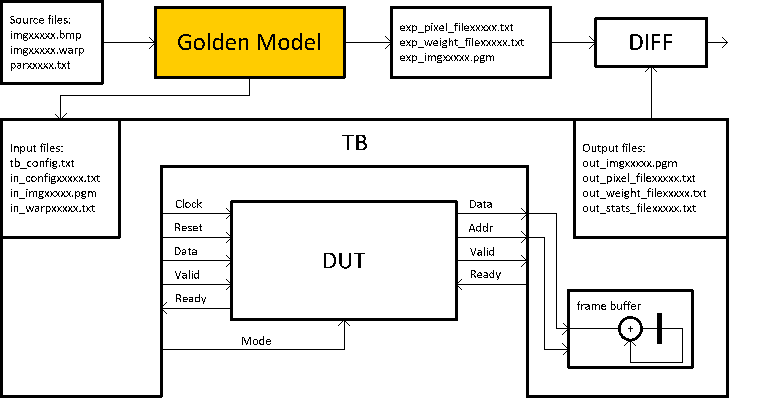
\includegraphics[width=\linewidth]{./figures/tb}
  \caption{Functional verification setup.}
  \label{fig:func_ver}
\end{figure}

\subsection{Design for Testability (DFT)}
\subsubsection{Automated Testpattern Generation}

\section{Results}
If you only have very few results, it might be a better approach to
insert them into this chapter (instead of putting the results into a
separate one).

%%%%%%%%%%%%%%%%%%%%%%%%%%%%%%%%%%%%%%%%%%%%%%%%%%%%%%%%%%%%%%%%%%%%%%%
%%%%%%%%%%%%%%%%%%%%%%%%%%%%%%%%%%%%%%%%%%%%%%%%%%%%%%%%%%%%%%%%%%%%%%%
%%%%%                                                                 %
%%%%%     <file_name>.tex                                             %
%%%%%                                                                 %
%%%%% Author:      <author>                                           %
%%%%% Created:     <date>                                             %
%%%%% Description: <description>                                      %
%%%%%                                                                 %
%%%%%%%%%%%%%%%%%%%%%%%%%%%%%%%%%%%%%%%%%%%%%%%%%%%%%%%%%%%%%%%%%%%%%%%
%%%%%%%%%%%%%%%%%%%%%%%%%%%%%%%%%%%%%%%%%%%%%%%%%%%%%%%%%%%%%%%%%%%%%%%

\chapter{Results}
If you have a large amount of results you can move them to this
separate chapter.

\section{First Section}


\section{Second Section}




%%%%%%%%%%%%%%%%%%%%%%%%%%%%%%%%%%%%%%%%%%%%%%%%%%%%%%%%%%%%%%%%%%%%%%%
%%%%%%%%%%%%%%%%%%%%%%%%%%%%%%%%%%%%%%%%%%%%%%%%%%%%%%%%%%%%%%%%%%%%%%%
%%%%%                                                                 %
%%%%%     <file_name>.tex                                             %
%%%%%                                                                 %
%%%%% Author:      <author>                                           %
%%%%% Created:     <date>                                             %
%%%%% Description: <description>                                      %
%%%%%                                                                 %
%%%%%%%%%%%%%%%%%%%%%%%%%%%%%%%%%%%%%%%%%%%%%%%%%%%%%%%%%%%%%%%%%%%%%%%
%%%%%%%%%%%%%%%%%%%%%%%%%%%%%%%%%%%%%%%%%%%%%%%%%%%%%%%%%%%%%%%%%%%%%%%

\chapter{Conclusion and Future Work}
Draw your conclusions from the results you achieved and summarize your
contributions. Comparisons (e.g., of hardware figures) with related
work are also appropriate here. Point out things that could or need to
be investigated further.

\section{First Section}


\section{Second Section}






%%%%%
%%%%% Start of additional parts.
%%%%%
\appendix

%%%%%%%%%%%%%%%%%%%%%%%%%%%%%%%%%%%%%%%%%%%%%%%%%%%%%%%%%%%%%%%%%%%%%%%
%%%%%%%%%%%%%%%%%%%%%%%%%%%%%%%%%%%%%%%%%%%%%%%%%%%%%%%%%%%%%%%%%%%%%%%
%%%%%                                                                 %
%%%%%     <file_name>.tex                                             %
%%%%%                                                                 %
%%%%% Author:      <author>                                           %
%%%%% Created:     <date>                                             %
%%%%% Description: <description>                                      %
%%%%%                                                                 %
%%%%%%%%%%%%%%%%%%%%%%%%%%%%%%%%%%%%%%%%%%%%%%%%%%%%%%%%%%%%%%%%%%%%%%%
%%%%%%%%%%%%%%%%%%%%%%%%%%%%%%%%%%%%%%%%%%%%%%%%%%%%%%%%%%%%%%%%%%%%%%%

\chapter{Task Description}
Include the task description \textbf{pdf} you got from your
assistant(s) with the \shell{\textbackslash includepdf} command.
% include the task description pdf!
%\includepdf[pages=-, turn=false, scale=0.9]{../../task/TaskDescription.pdf}


\chapter{Declaration of Originality}\label{chap:originality}
Include the declaration of authorship with the \shell{\textbackslash
  includepdf} command (sign it and scan it). For more information
about plagiarism, please visit
\url{https://www.ethz.ch/students/en/studies/performance-assessments/plagiarism.html}

\begin{itemize}
\item \textbf{English version:}
  \url{https://www.ethz.ch/content/dam/ethz/main/education/rechtliches-abschluesse/leistungskontrollen/declaration-originality.pdf}
\item \textbf{German version:}
  \url{https://www.ethz.ch/content/dam/ethz/main/education/rechtliches-abschluesse/leistungskontrollen/plagiat-eigenstaendigkeitserklaerung.pdf}
\end{itemize}

% include the signed declaration of authorship!
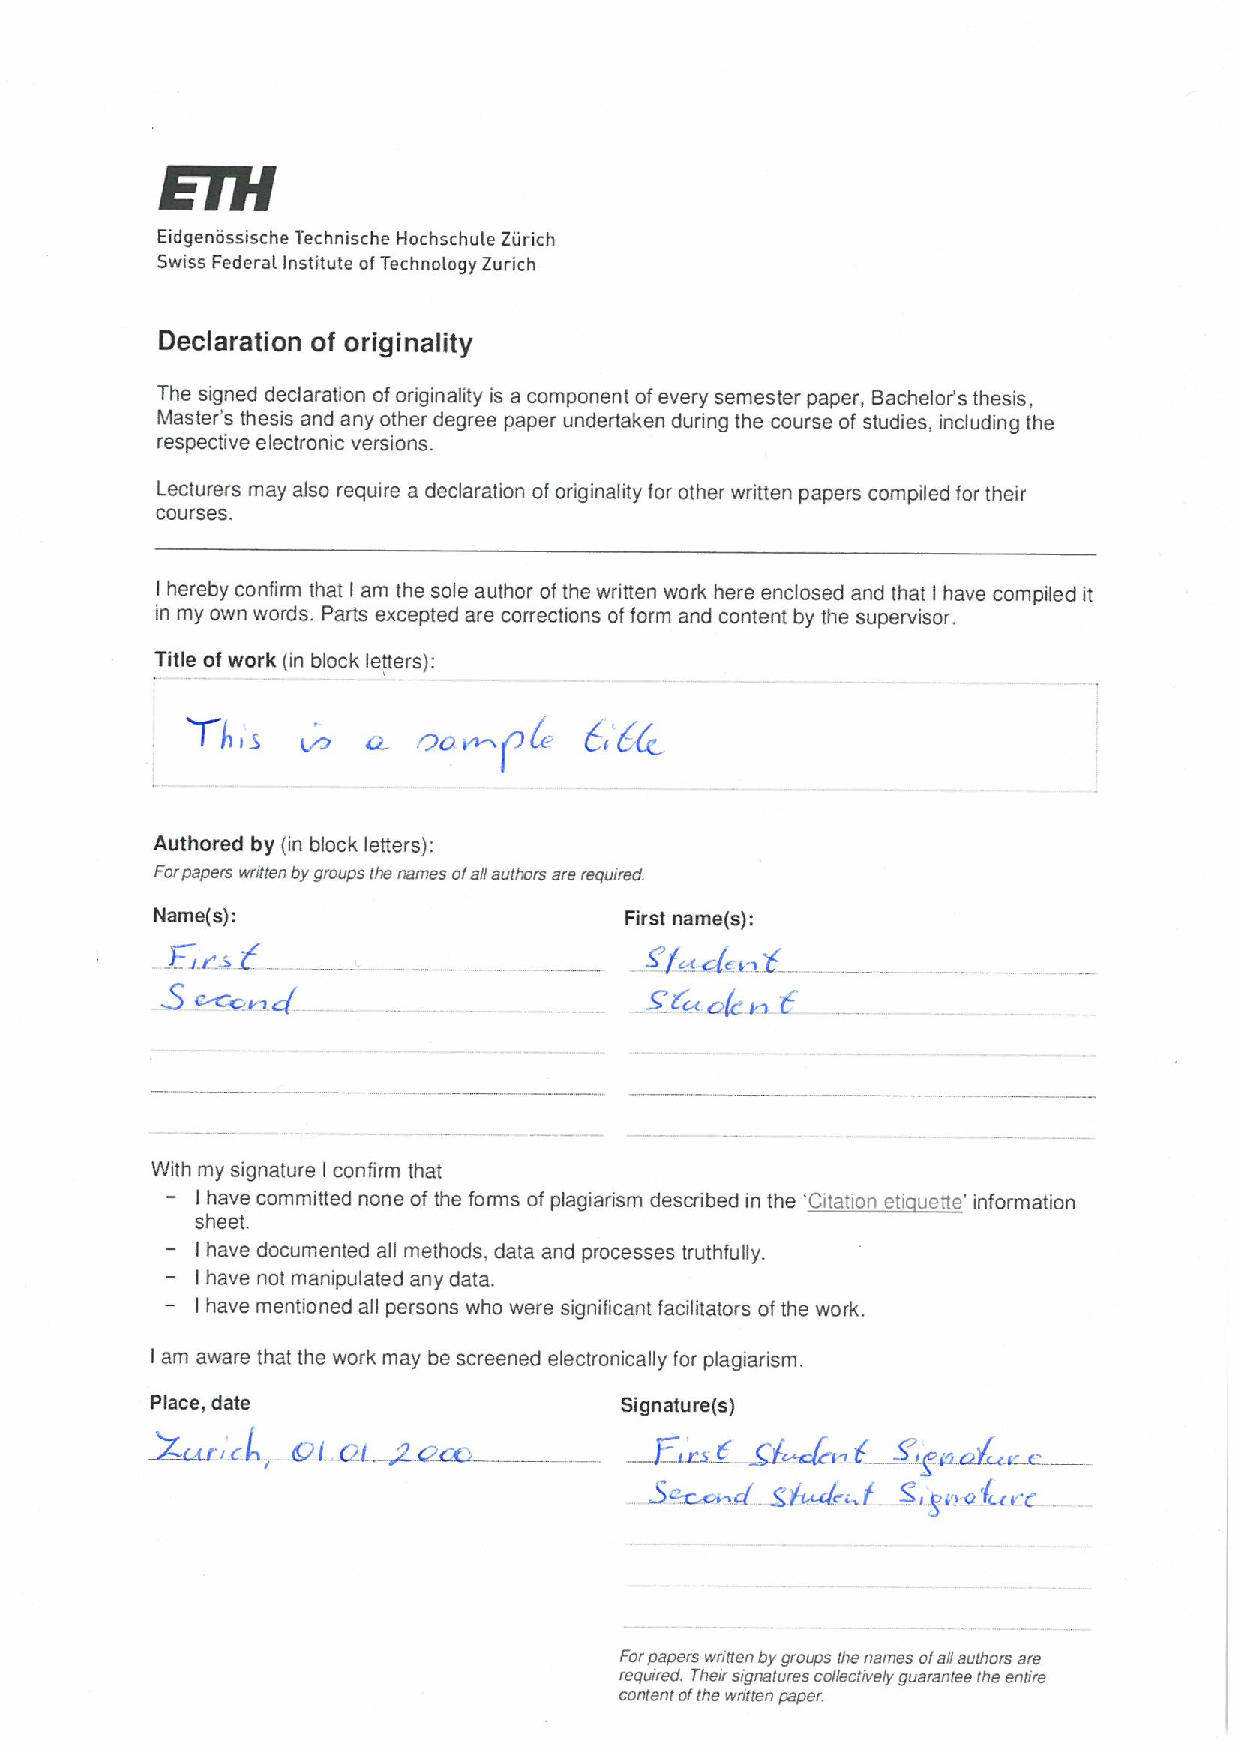
\includepdf[pages=-, turn=false, scale=0.9]{./figures/declaration_of_originality}


\chapter{File Structure}
Describe how the project directories/files are organized, e.g.:

\begin{flushleft}
\dirtree{%
.1 /.
  .2 README \DTcomment{A README with some general information about the project.}.
  .2 01\_report \DTcomment{The source files of the project report.}.
  .2 02\_presentation \DTcomment{The source files of the presentation.}.
  .2 03\_designflow \DTcomment{Some designflow-specific files.}.
}
\end{flushleft}

What needs to be done to run an RTL simulation (stimuli generation,
compilation...)?


\chapter{Datasets}
If you have a data set comprising several test images, you could
depict and describe them here. Use a simple naming scheme such that
you can easily refer to certain elements of this data set in the text.


\chapter{More Evaluation Results}
If you conducted an extensive evaluation you could move surplus
graphs/results to the appendix.


\chapter{Algorithms / Tables}
Large algorithm boxes and tables may clutter your chapters and impair
the readability. If they are not very important, consider moving them
to the appendix as well.


\chapter{ASIC Datasheet ($<$Chipname$>$)}

If you have designed an \gls{asic} during your work, you should
include a datasheet for your chip into the report. As soon as you
start testing your fabricated chip, you will be glad to have such a
datasheet. An example structure of such a datasheet is given in the
following. For more inspirations on what you may include in your
datasheet, have a look at the datasheet of a commercial \gls{ic}.

\minitoc

\section{Features}
\begin{itemize}
\item Lorem ipsum dolor sit amet, ...
\item Lorem ipsum dolor sit amet, ...
\item Lorem ipsum dolor sit amet, ...
\item Lorem ipsum dolor sit amet, ...
\end{itemize}

\section{Applications}
\lipsum[2]

\section{Description}
\lipsum[2]

\section{Packaging}
\lipsum[2]

\section{Bonding Diagram}
\lipsum[2]

\begin{figure}[htbp]
  \centering 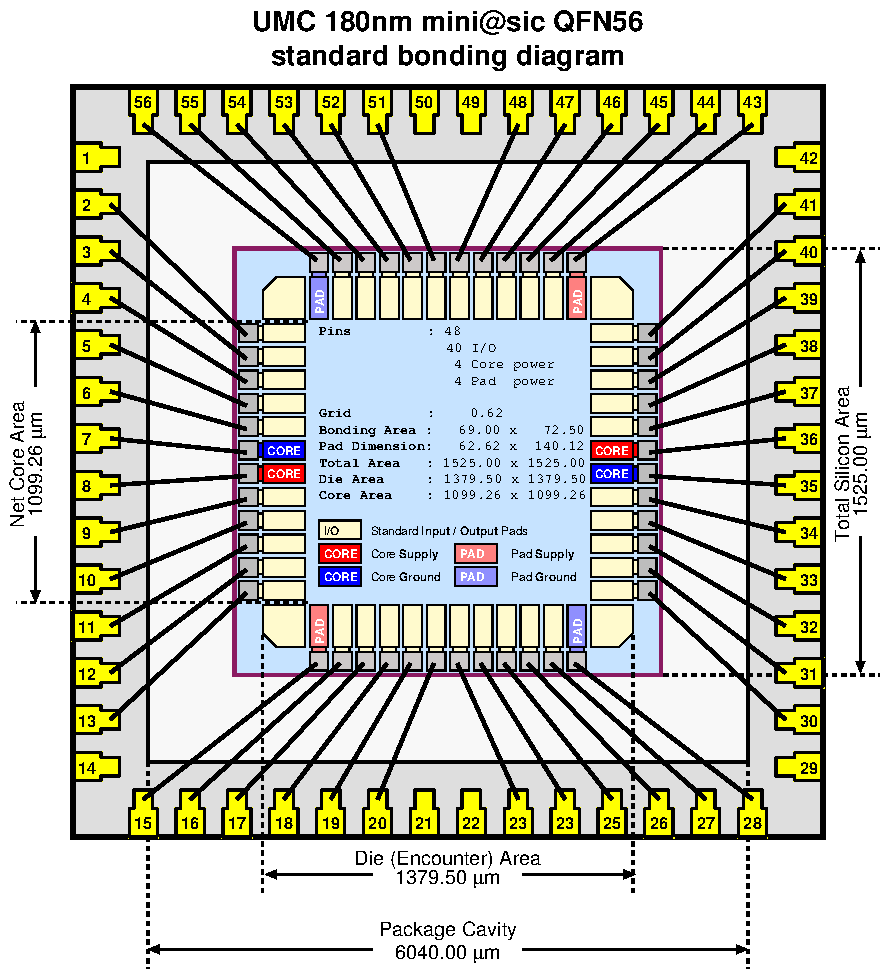
\includegraphics[width=0.9\textwidth]{./figures/qfn56_180_std}
  \caption{Bonding diagram.}
\end{figure}

\section{Pin Map}
\lipsum[2]

\begin{figure}[htbp]
  \centering 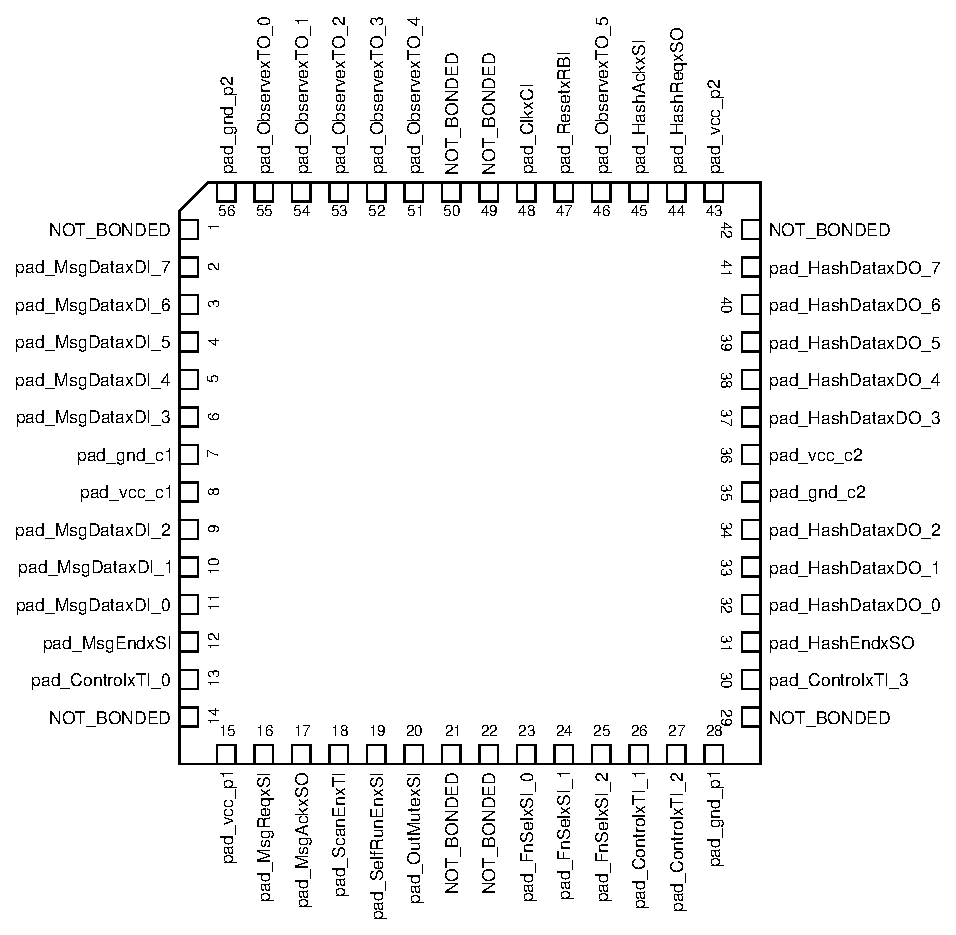
\includegraphics[width=1.0\textwidth]{./figures/asic_pinout}
  \caption{$<$Chipname$>$ pinout.}
\end{figure}

\section{Pin Description}
\lipsum[2]

\section{Interface Description}
\lipsum[2]

\section{Register Map}
\lipsum[2]

\section{Operation Modes}
\lipsum[2]

\subsection{Functional Modes}
\subsection{Test Modes}

\section{Electrical Specifications}
\lipsum[2]
\subsection{Recommended Operating Regions}
\subsection{Absolute Maximum Ratings}

%%%%%%%%%%%%%%%%%%%%%%%%%%%%%%%%%%%%%%%%%%%%%%%%%%%%%%%%%%%%%%%%%%%%%%%
%%%%%%%%%%%%%%%%%%%%%%%%%%%%%%%%%%%%%%%%%%%%%%%%%%%%%%%%%%%%%%%%%%%%%%%
%%%%%                                                                 %
%%%%%     z_02_directories.tex                                        %
%%%%%                                                                 %
%%%%% Author:      Michael Muehlberghuber (<mbgh@iis.ee.ethz.ch>      %
%%%%% Created:     01.07.2012                                         %
%%%%% Description: A description of all files and directories         %
%%%%%              contained within this LaTeX framework.             %
%%%%%                                                                 %
%%%%%                                                                 %
%%%%% History:                                                        %
%%%%%%%%%%%%%%                                                        %
%%%%%                                                                 %
%%%%% 01-Jul-2012 (Michael Muehlberghuber - mbgh@iis.ee.ethz.ch):     %
%%%%% *) Created initial version.                                     %
%%%%%                                                                 %
%%%%%%%%%%%%%%%%%%%%%%%%%%%%%%%%%%%%%%%%%%%%%%%%%%%%%%%%%%%%%%%%%%%%%%%
%%%%%%%%%%%%%%%%%%%%%%%%%%%%%%%%%%%%%%%%%%%%%%%%%%%%%%%%%%%%%%%%%%%%%%%

\chapter{The Template Directory Structure}

This \LaTeX{} framework suitable for creating reports spreads over
various directories and files. In order to give you a short overview
of this structure, the respective directories and the contained files
are described in the following:

\begin{flushleft}
\dirtree{%
.1 /.
  .2 README \DTcomment{README file with a quick start guide.}.
  .2 Makefile \DTcomment{Makefile with some \LaTeX{} related build targets.}.
  .2 report\_template.tex \DTcomment{The main \LaTeX{} file of the report document, which further loads other (content) files.}.
  .2 bib \DTcomment{Contains bibliography related files.}.
    .3 main.bib \DTcomment{Bibliography file.}.
  .2 content \DTcomment{Contains the actual source files of your report.}.
    .3 *$.$tex \DTcomment{Here, multiple content files are provided.}.
  .2 figures \DTcomment{Contains the images which are loaded during your report.}.
    .3 eth\_logo.* \DTcomment{ETH logo in \gls{eps} and \gls{pdf} format.}.
    .3 titlepage\_logo.* \DTcomment{Titlepage logo in \gls{eps} and \gls{pdf} format.}.
    .3 asic\_pinout.* \DTcomment{Sample pinout of an \gls{asic} in \gls{eps} and \gls{pdf} format.}.
  .2 figures\_raw \DTcomment{Contains the raw sources of your figures.}.
    .3 titlepage\_logo.obj \DTcomment{Tgif titlepage logo source.}.
  .2 glossaries \DTcomment{Contains glossaries.}.
    .3 glossaries.tex \DTcomment{The glossaries file containing both the entries of the list of acronym entries and the entries of the main glossary.}.
  .2 preamble \DTcomment{Contains preamble information of the document.}.
    .3 preamble.tex \DTcomment{Preamble of the report document.}.
}
\end{flushleft}


%%% Local Variables: 
%%% mode: latex
%%% TeX-master: "../report_template"
%%% End: 

%%%%%%%%%%%%%%%%%%%%%%%%%%%%%%%%%%%%%%%%%%%%%%%%%%%%%%%%%%%%%%%%%%%%%%%
%%%%%%%%%%%%%%%%%%%%%%%%%%%%%%%%%%%%%%%%%%%%%%%%%%%%%%%%%%%%%%%%%%%%%%%
%%%%%                                                                 %
%%%%%     z_03_latex_tips.tex                                         %
%%%%%                                                                 %
%%%%% Author:      Michael Muehlberghuber (<mbgh@iis.ee.ethz.ch>      %
%%%%% Created:     01.07.2012                                         %
%%%%% Description: Some LaTeX-specific writing tips                   %
%%%%%                                                                 %
%%%%%                                                                 %
%%%%% History:                                                        %
%%%%%%%%%%%%%%                                                        %
%%%%%                                                                 %
%%%%% 01-Jul-2012 (Michael Muehlberghuber - mbgh@iis.ee.ethz.ch):     %
%%%%% *) Created initial version.                                     %
%%%%%                                                                 %
%%%%%%%%%%%%%%%%%%%%%%%%%%%%%%%%%%%%%%%%%%%%%%%%%%%%%%%%%%%%%%%%%%%%%%%
%%%%%%%%%%%%%%%%%%%%%%%%%%%%%%%%%%%%%%%%%%%%%%%%%%%%%%%%%%%%%%%%%%%%%%%

\chapter{\LaTeX{} Tips}

Writing a report with \LaTeX{} may not be as intuitive as it is the
case with \gls{wysiwyg} editors. Especially if you are using \LaTeX{}
(more or less) the first time, some problems with the syntax will
occur. In general, the present document should already serve as a good
starting point for your report and in the best case you only have to
insert the content of your project based on this framework.

Nevertheless, I will try to give some useful tips with regard to
\LaTeX{} throughout the next sections, which may help you to increase
the quality of your documents even further. If you want to use any of
the presented ideas, simply copy the \LaTeX{} source code of the
appropriate section to your on document and adapt it accordingly.


\section{Compiling a \LaTeX{} Document}
\label{sec:compiling}

Basically, either \shell{latex} or \shell{pdflatex} can be used in
order to generate the document output in \gls{dvi} or \gls{pdf}
format, respectively. Throughout this section I will solely use the
\shell{pdflatex} command for demonstration purposes (if you prefer a
DVI document, just replace the \shell{pdflatex} command by
\shell{latex}0).

Compiling a latex document at the \gls{iis} computers is, in general,
as simple as executing the following command in a UNIX terminal
window:

\begin{shellenv}
pdflatex <document_name>
\end{shellenv}

Currently\footnote{State: July 2012} a \TeX{} Live version from the
year 2008 is the default distribution at the \gls{iis}. In order to
use the present \LaTeX{} framework for your report, you have to use a
more up-to-date version of \TeX{} Live, because the framework uses
some \LaTeX{} packages which are not part of the 2008 version. I
suggest using the 2011 version of \TeX{} Live. The simplest way to
check that you can build the report template successfully, is by
executing:

\begin{shellenv}
pdflatex-2011 report_template.tex
\end{shellenv}

This should (re)generate the \gls{pdf} output of the report template,
i.e., the file you are currently reading through. If typing in the
\shell{-2011} postfix becomes annoying for you, you may add aliases
into your \file{.cshrc} as follows:

\begin{shellenv}
alias latex 'latex-2011'
alias pdflatex 'pdflatex-2011'
\end{shellenv}

If you also want to (re)build the glossaries (maybe you have added
some acronyms or the like), you have to compile your report together
with the glossaries as follows:

\begin{shellenv}
pdflatex-2011 your_report.tex
makeglossaries-2011 your_report
pdflatex-2011 your_report.tex
\end{shellenv}

Furthermore, when you modify the references of your report (within the
bibliography file), you also have to (re)run \textsc{Bib}\TeX{} in
order to update your bibliography, i.e.:

\begin{shellenv}
pdflatex-2011 your_report.tex
bibtex-2011 your_report
pdflatex-2011 your_report.tex
pdflatex-2011 your_report.tex
\end{shellenv}


\section{Figures}
\label{sec:figures}

In order to include an image into your report (as it has been done
within in the previous sample chapters), you may use the
\texttt{figure} floating environment. With that, \LaTeX{} will take
care of placing them nicely and you can focus on the actual content of
your document. Figure~\ref{fig:std_eth_logo} shows an example of how
to insert a single figure.

\begin{figure}[htbp]
 \centering
\includegraphics[width=0.4\linewidth]{./figures/eth_logo}
 \caption{Standard ETH logo.}
 \label{fig:std_eth_logo}
\end{figure}

If you want to place multiple figures side-by-side, you can do this
with the use of \texttt{minipages}. Figure~\ref{fig:left_eth_logo} and
\ref{fig:right_eth_logo} illustrates an example.

\begin{figure}[htbp]
 \begin{minipage}[t]{0.45\linewidth}
  \centering
\includegraphics[width=1.0\linewidth]{./figures/eth_logo}
  \caption{Left ETH logo.}
  \label{fig:left_eth_logo}
 \end{minipage}\hfill
 \begin{minipage}[t]{0.45\linewidth}
  \centering
\includegraphics[width=1.0\linewidth]{./figures/eth_logo}
  \caption{Right ETH logo.}
  \label{fig:right_eth_logo}
 \end{minipage}
\end{figure}

In order to create a single figure with multiple subfigures, you can
do this as presented in Figure~\ref{fig:eth_logo_sub}

\begin{figure}[htbp]
 \centering
 \subfloat[Left ETH logo.]{
\includegraphics[width=0.3\textwidth]{./figures/eth_logo}}\hfill
 \subfloat[Center ETH logo.]{
\includegraphics[width=0.3\textwidth]{./figures/eth_logo}}\hfill
 \subfloat[Right ETH logo.]{
\includegraphics[width=0.3\textwidth]{./figures/eth_logo}}
 \caption{Multiple ETH logos as subfigures.}
 \label{fig:eth_logo_sub}
\end{figure}


\section{Tables}
\label{sec:tables}

Tables in \LaTeX{} allow you to present your results quite
nicely. Table~\ref{tab:std_table} shows a standard table.

\begin{table}[htbp]
 \caption{Standard table.}
 \label{tab:std_table}
 \centering\begin{tabular}{@{}lcr@{}} \toprule
  \textbf{Row 1 - Column 1} & \textbf{Row 1 - Column 2} & \textbf{Row 1 - Column 3} \\ \midrule
  Row 2 - Column 1 & Row 2 - Column 2 & Row 2 - Column 3 \\
  Row 3 - Column 1 & Row 3 - Column 2 & Row 3 - Column 3 \\
  Row 4 - Column 1 & Row 4 - Column 2 & Row 4 - Column 3 \\ \bottomrule
 \end{tabular}
\end{table}

Sometimes you may want to add a table which stretches one of its
columns in order to reach the full width of the document. Such an
example is shown in Table~\ref{tab:stretched_table}.

\begin{table}[htbp]
 \caption{Stretched table.}
 \label{tab:stretched_table}
 \centering\begin{tabularx}{1.0\linewidth}{@{}Xcr@{}} \toprule
  \textbf{Row 1 - Column 1} & \textbf{Row 1 - Column 2} & \textbf{Row 1 - Column 3} \\ \midrule
  Row 2 - Column 1 & Row 2 - Column 2 & Row 2 - Column 3 \\
  Row 3 - Column 1 & Row 3 - Column 2 & Row 3 - Column 3 \\
  Row 4 - Column 1 & Row 4 - Column 2 & Row 4 - Column 3 \\ \bottomrule
 \end{tabularx}
\end{table}

If you need to place two tables next to each other, you may use an
approach based on \texttt{minipages} as shown in Table~\ref{tbl:left}
and Table~\ref{tbl:right}.

\begin{figure}
  \begin{minipage}{0.49\textwidth}
    \captionof{table}{Left table.}
    \label{tbl:left}
    \centering\begin{tabular}{@{}lr@{}} \toprule
      Row 1 - Column 1 & Row 1 - Column 2 \\ \midrule
      Row 2 - Column 1 & Row 2 - Column 2 \\
      Row 3 - Column 1 & Row 3 - Column 2 \\
      Row 4 - Column 1 & Row 4 - Column 2 \\ \bottomrule
    \end{tabular}
  \end{minipage} \hfill
  %
  \begin{minipage}{0.49\textwidth}
    \captionof{table}{Right table.}
    \label{tbl:right}
    \centering\begin{tabular}{@{}lr@{}} \toprule
      Row 1 - Column 1 & Row 1 - Column 2 \\ \midrule
      Row 2 - Column 1 & Row 2 - Column 2 \\
      Row 3 - Column 1 & Row 3 - Column 2 \\
      Row 4 - Column 1 & Row 4 - Column 2 \\ \bottomrule
    \end{tabular}
  \end{minipage}
\end{figure}

\section{Creating Glossaries}

In order to generate a glossary within your report (e.g., a list of
acronyms or an actual glossary), take a look into the file
\texttt{glossaries.tex}. There, you will find some examples on how to
define an acronym as well as a glossary entry. If you want to
reference one of the acronyms within your report, you can do it the
same way as I did it with the \gls{led} right here (just take a look
into the source code).

As already mentioned in Section~\ref{sec:compiling}, you have to
rebuild your glossaries in order to display changes. For that, you
first have to build your document using \texttt{latex-2011} or
\texttt{pdflatex-2011} in a shell window, or the \textit{build-button}
in your preferred \LaTeX{} editor GUI. Next, you have to call
\texttt{makeglossaries-2011 \parameter{file\_name}} in a shell
window\footnote{The \texttt{makeglossaries} script is a Perl script
  available at the IIS computer system and should also be part of most
  \TeX{} distributions.}, followed by another build process of your
main source file, i.e.:

\begin{shellenv}
pdflatex-2011 your_report.tex
makeglossaries-2011 your_report
pdflatex-2011 your_report.tex
\end{shellenv}


\section{Creating Algorithm Boxes}

Algorithm boxes in \LaTeX{} allow you to present your algorithms in
pseudo code as shown in the following example:

\begin{algorithm}
  \SetKwData{Left}{left}\SetKwData{This}{this}\SetKwData{Up}{up}
  \SetKwFunction{Union}{Union}\SetKwFunction{FindCompress}{FindCompress}
  \SetKwInOut{Input}{input}\SetKwInOut{Output}{output}

  \Input{A bitmap $Im$ of size $w\times l$}
  \Output{A partition of the bitmap}
  \BlankLine
  \emph{special treatment of the first line}\;
  \For{$i\leftarrow 2$ \KwTo $l$}{
    \emph{special treatment of the first element of line $i$}\;
    \For{$j\leftarrow 2$ \KwTo $w$}{\label{forins}
      \Left$\leftarrow$ \FindCompress{$Im[i,j-1]$}\;
      \Up$\leftarrow$ \FindCompress{$Im[i-1,]$}\;
      \This$\leftarrow$ \FindCompress{$Im[i,j]$}\;
      \If(\tcp*[h]{O(\Left,\This)==1}){\Left compatible with \This}{\label{lt}
        \lIf{\Left $<$ \This}{\Union{\Left,\This}}\;
        \lElse{\Union{\This,\Left}\;}
      }
      \If(\tcp*[f]{O(\Up,\This)==1}){\Up compatible with \This}{\label{ut}
        \lIf{\Up $<$ \This}{\Union{\Up,\This}}\;
        \tcp{\This is put under \Up to keep tree as flat as possible}\label{cmt}
        \lElse{\Union{\This,\Up}}\tcp*[r]{\This linked to \Up}\label{lelse}
      }
    }
    \lForEach{element $e$ of the line $i$}{\FindCompress{p}}
  }
  \caption{disjoint decomposition}\label{algo_disjdecomp}
\end{algorithm}


% \section{Citing}


% \section{Units}

%%% Local Variables:
%%% mode: latex
%%% TeX-master: "../report_template"
%%% End:

%%%%%%%%%%%%%%%%%%%%%%%%%%%%%%%%%%%%%%%%%%%%%%%%%%%%%%%%%%%%%%%%%%%%%%%
%%%%%%%%%%%%%%%%%%%%%%%%%%%%%%%%%%%%%%%%%%%%%%%%%%%%%%%%%%%%%%%%%%%%%%%
%%%%%                                                                 %
%%%%%     z_04_writing_tips.tex                                       %
%%%%%                                                                 %
%%%%% Author:      Michael Muehlberghuber (<mbgh@iis.ee.ethz.ch>      %
%%%%% Created:     01.07.2012                                         %
%%%%% Description: Some Writing-specific tips in general.             %
%%%%%                                                                 %
%%%%% History:                                                        %
%%%%%%%%%%%%%%                                                        %
%%%%%                                                                 %
%%%%% 01-Jul-2012 (Michael Muehlberghuber - mbgh@iis.ee.ethz.ch):     %
%%%%% *) Created initial version.                                     %
%%%%%                                                                 %
%%%%%%%%%%%%%%%%%%%%%%%%%%%%%%%%%%%%%%%%%%%%%%%%%%%%%%%%%%%%%%%%%%%%%%%
%%%%%%%%%%%%%%%%%%%%%%%%%%%%%%%%%%%%%%%%%%%%%%%%%%%%%%%%%%%%%%%%%%%%%%%

\chapter{General Writing Guidelines}

As soon as you get familiar with the syntax of \LaTeX{} (and I can
promise you, you will get familiar with it quite quickly as soon as
you start writing your reports with \LaTeX{}), some more general
writing tips might become of interest for your. Therefore, I collected
a few general writing guidlines in the following sections, some of
them with regard to \LaTeX{}, some of them not.

\paragraph{Placement of Floating Environments}
Figures and tables are the two most prominent examples for floating
environments. Although the figure examples presented in
Section~\ref{sec:figures} use \texttt{[htbp]} to tell \LaTeX{} how to
place them, you should normally only use the \texttt{h} parameter if
you really require it. Since \LaTeX{} then at first tries to place the
figure at the same position as its source code, this somehow
contradicts with the actual purpose of the \texttt{figure}
environment. So, in general, try to place floating environments using
one of the following parameters:

\begin{description}
\item[t] Place the floating environment on \textbf{t}op of a page.
\item[b] Place the floating environment on the \textbf{b}ottom of a
  page.
\item[p] Puts the floating environment on a single \textit{floating
    \textbf{p}age} with other floating environments.
\end{description}


\paragraph{Positioning of Figure and Table Captions}
Captions of figures are, in general, placed below the actual figure,
whereas captions of tables should be placed on top of
them. Section~\ref{sec:figures} and \ref{sec:tables} contain some
examples for figures and tables, including correct placement of
captions.


\paragraph{Avoid Unneccessary \LaTeX{} Packages}
Although there are so many ``cool'' \LaTeX{} packages available
everywhere on the Internet, try to use only those, which you really
require. The main problem with loading too many, more or less unknown,
packages is that some of them might redefine some commands, etc.,
which are used by another package which asumes that command to be the
original one. Keeping track of these changes and the relations between
different packages, is quite annoying and takes quite a lot of
time. Hence, keep your preamble simple with regard to packages.


\paragraph{Make Use of Vector Drawings}
Since \LaTeX{} handles vector drawings pretty good and their
scalability allows you to print them in any resolution, prefer them
compared to their pixel counterparts and use them whenever possible.

% \paragraph{Equations Within the ``Text-Flow''}

% \paragraph{Punctuation within Captions}
% \begin{itemize}
%  \item No second fullstop when ending sentences with abbreviations like
%  etc.
% \end{itemize}

%%% Local Variables:
%%% mode: latex
%%% TeX-master: "../report_template"
%%% End:


\backmatter

% Print the main glossary.
\printglossary[type=main,title=Glossary]


% Print the bibliography.
\nocite*{} % Print non-cited references as well.
\bibliographystyle{IEEEtran}
\bibliography{IEEEabrv,./bib/main}


\end{document}
%%%%%%%%%%%%%%%%%%%%%%%%%%%%%%%%%%%%%%%%%%%%%%%%%%%%%%%%%%%%%%%%%%%%%%%
%%%%%                                                                 %
%%%%%     End of Document                                             %
%%%%%                                                                 %
%%%%%%%%%%%%%%%%%%%%%%%%%%%%%%%%%%%%%%%%%%%%%%%%%%%%%%%%%%%%%%%%%%%%%%%
